% Drawing 79/14-4 -- folder 79, batch 14, archive page 280 (PDF page 281).
% Transcription: dans la marge de gauche, au crayon léger, un octaèdre en perspective.
% Kind: octahedron in perspective (light pencil). Method 2 (schematic redraw from the facsimile). Status: partial.
% Notes: Light pencil octahedron: apex T, bottom B, equator L, F, R, K. Which strokes are hidden is not marked; the edges are a reading of faint, doubled strokes (notably K-L and the back edges). Not encoded: the page does not fix the incidences with certainty.
% Coordinates: 1 unit = 1 mm = 1/100 of the crop width (bbox in page fractions: [0.08, 0.69, 0.22, 0.8]).
% Redrawn by Claude (claude-opus-5-5), issue #73, 2026-11-07; not checked by a human; not compiled (no TeX in the session).
% Rights: reproduces part of the work -- behind RENDER_TRANSCRIPTS, never published by itself.
\documentclass[tikz,border=3pt]{standalone}
\usepackage{amsmath,amssymb}
\usetikzlibrary{patterns,arrows.meta}
\tikzset{pencil/.style={black!45}, struck/.style={black!35}, mark/.style={circle,draw,inner sep=1.3pt}, pt/.style={circle,fill,inner sep=0.9pt}, opt/.style={circle,draw,fill=white,inner sep=1.1pt}}
\begin{document}
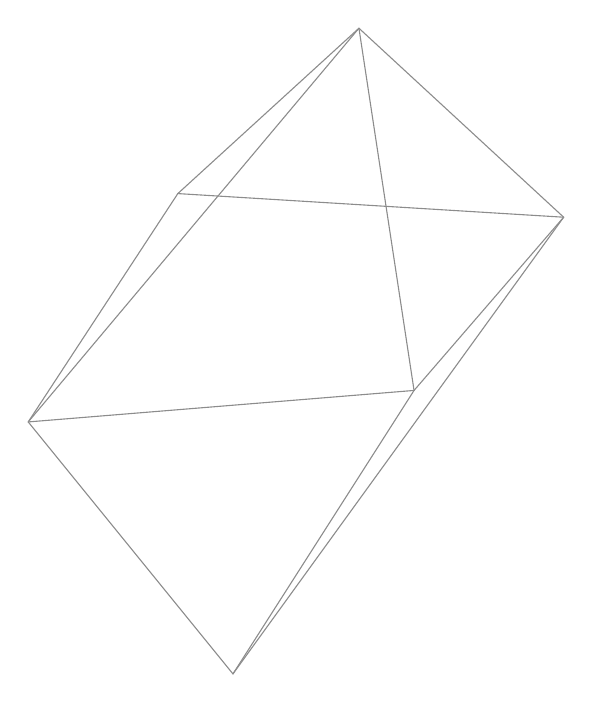
\begin{tikzpicture}[x=1mm,y=1mm,line cap=round,line join=round,font=\scriptsize]
\draw[pencil] (61,-21) -- (19,-71);
\draw[pencil] (61,-21) -- (87,-45);
\draw[pencil] (61,-21) -- (68,-67);
\draw[pencil] (61,-21) -- (38,-42);
\draw[pencil] (45,-103) -- (19,-71);
\draw[pencil] (45,-103) -- (87,-45);
\draw[pencil] (45,-103) -- (68,-67);
\draw[pencil] (19,-71) -- (68,-67);
\draw[pencil] (68,-67) -- (87,-45);
\draw[pencil] (87,-45) -- (38,-42);
\draw[pencil] (38,-42) -- (19,-71);
\end{tikzpicture}
\end{document}
